%%%%%%%%%%%%%%%%%%%%%%%%%%%%%%%%%%%%%%%%%
% Arsclassica Article
% LaTeX Template
% Version 1.1 (1/8/17)
%
% This template has been downloaded from:
% http://www.LaTeXTemplates.com
%
% Original author:
% Lorenzo Pantieri (http://www.lorenzopantieri.net) with extensive modifications by:
% Vel (vel@latextemplates.com)
%
% License:
% CC BY-NC-SA 3.0 (http://creativecommons.org/licenses/by-nc-sa/3.0/)
%
%%%%%%%%%%%%%%%%%%%%%%%%%%%%%%%%%%%%%%%%%

%----------------------------------------------------------------------------------------
%	PACKAGES AND OTHER DOCUMENT CONFIGURATIONS
%----------------------------------------------------------------------------------------

\documentclass[
10pt, % Main document font size
a4paper, % Paper type, use 'letterpaper' for US Letter paper
oneside, % One page layout (no page indentation)
%twoside, % Two page layout (page indentation for binding and different headers)
headinclude,footinclude, % Extra spacing for the header and footer
BCOR5mm, % Binding correction
]{scrartcl}


\usepackage{natbib}
\usepackage{float}

%%%%%%%%%%%%%%%%%%%%%%%%%%%%%%%%%%%%%%%%%
% Arsclassica Article
% Structure Specification File
%
% This file has been downloaded from:
% http://www.LaTeXTemplates.com
%
% Original author:
% Lorenzo Pantieri (http://www.lorenzopantieri.net) with extensive modifications by:
% Vel (vel@latextemplates.com)
%
% License:
% CC BY-NC-SA 3.0 (http://creativecommons.org/licenses/by-nc-sa/3.0/)
%
%%%%%%%%%%%%%%%%%%%%%%%%%%%%%%%%%%%%%%%%%

%----------------------------------------------------------------------------------------
%	REQUIRED PACKAGES
%----------------------------------------------------------------------------------------

\usepackage[
nochapters, % Turn off chapters since this is an article        
beramono, % Use the Bera Mono font for monospaced text (\texttt)
eulermath,% Use the Euler font for mathematics
pdfspacing, % Makes use of pdftex’ letter spacing capabilities via the microtype package
dottedtoc % Dotted lines leading to the page numbers in the table of contents
]{classicthesis} % The layout is based on the Classic Thesis style

\usepackage{arsclassica} % Modifies the Classic Thesis package

\usepackage[T1]{fontenc} % Use 8-bit encoding that has 256 glyphs

\usepackage[utf8]{inputenc} % Required for including letters with accents

\usepackage{graphicx} % Required for including images
\graphicspath{{Figures/}} % Set the default folder for images

\usepackage{enumitem} % Required for manipulating the whitespace between and within lists

\usepackage{lipsum} % Used for inserting dummy 'Lorem ipsum' text into the template

\usepackage{subfig} % Required for creating figures with multiple parts (subfigures)

\usepackage{amsmath,amssymb,amsthm} % For including math equations, theorems, symbols, etc

\usepackage{varioref} % More descriptive referencing

%----------------------------------------------------------------------------------------
%	THEOREM STYLES
%---------------------------------------------------------------------------------------

\theoremstyle{definition} % Define theorem styles here based on the definition style (used for definitions and examples)
\newtheorem{definition}{Definition}

\theoremstyle{plain} % Define theorem styles here based on the plain style (used for theorems, lemmas, propositions)
\newtheorem{theorem}{Theorem}

\theoremstyle{remark} % Define theorem styles here based on the remark style (used for remarks and notes)

%----------------------------------------------------------------------------------------
%	HYPERLINKS
%---------------------------------------------------------------------------------------

\hypersetup{
%draft, % Uncomment to remove all links (useful for printing in black and white)
colorlinks=true, breaklinks=true, bookmarks=true,bookmarksnumbered,
urlcolor=webbrown, linkcolor=RoyalBlue, citecolor=webgreen, % Link colors
pdftitle={}, % PDF title
pdfauthor={\textcopyright}, % PDF Author
pdfsubject={}, % PDF Subject
pdfkeywords={}, % PDF Keywords
pdfcreator={pdfLaTeX}, % PDF Creator
pdfproducer={LaTeX with hyperref and ClassicThesis} % PDF producer
} % Include the structure.tex file which specified the document structure and layout

\hyphenation{Fortran hy-phen-ation} % Specify custom hyphenation points in words with dashes where you would like hyphenation to occur, or alternatively, don't put any dashes in a word to stop hyphenation altogether

%----------------------------------------------------------------------------------------
%	TITLE AND AUTHOR(S)
%----------------------------------------------------------------------------------------

\title{\normalfont\spacedallcaps{Effectiveness of Portfolio Rebalancing from An Empirical Standpoint}} % The article title

%\subtitle{Subtitle} % Uncomment to display a subtitle

\author{Shan Tao, Xiang Li, Zhibo Wang} % The article author(s) - author affiliations need to be specified in the AUTHOR AFFILIATIONS block

\date{\today} % An optional date to appear under the author(s)

%----------------------------------------------------------------------------------------

\begin{document}

%----------------------------------------------------------------------------------------
%	HEADERS
%----------------------------------------------------------------------------------------

\renewcommand{\sectionmark}[1]{\markright{\spacedlowsmallcaps{#1}}} % The header for all pages (oneside) or for even pages (twoside)
%\renewcommand{\subsectionmark}[1]{\markright{\thesubsection~#1}} % Uncomment when using the twoside option - this modifies the header on odd pages
\lehead{\mbox{\llap{\small\thepage\kern1em\color{halfgray} \vline}\color{halfgray}\hspace{0.5em}\rightmark\hfil}} % The header style

\pagestyle{scrheadings} % Enable the headers specified in this block

%----------------------------------------------------------------------------------------
%	TABLE OF CONTENTS & LISTS OF FIGURES AND TABLES
%----------------------------------------------------------------------------------------

\maketitle % Print the title/author/date block

\setcounter{tocdepth}{2} % Set the depth of the table of contents to show sections and subsections only

\tableofcontents % Print the table of contents

\listoffigures % Print the list of figures

\listoftables % Print the list of tables

%----------------------------------------------------------------------------------------
%	ABSTRACT
%----------------------------------------------------------------------------------------

\section*{Abstract} % This section will not appear in the table of contents due to the star (\section*)



%----------------------------------------------------------------------------------------
%	AUTHOR AFFILIATIONS
%----------------------------------------------------------------------------------------


%----------------------------------------------------------------------------------------

\newpage % Start the article content on the second page, remove this if you have a longer abstract that goes onto the second page

%----------------------------------------------------------------------------------------
%	INTRODUCTION
%----------------------------------------------------------------------------------------

\section{Introduction}
Rebalancing is an essential branch of the portfolio management theory. As for holding positions of portfolios, the manager should always aim at the tradeoff between risk and return in the dynamic financial market to improve the performance. Strategies including buy-and-hold and rebalancing could be effective tools to achieve the goal to maximize the portfolio value. Rebalancing is a process in which the investor will reset the weights of assets contained in the portfolio in order to make them reinstate fixed market value
proportions, while buy-and-hold strategy is more direct and easier: the investor will buy the assets and build the portfolio, then just hold them without any rebalancing. There is common belief that periodical rebalancing strategy provides more benefits than buy-and-hold and this could be concluded as “the rebalancing bonus” originated by William Bernstein(1996). However, it is still a heated issue to discuss which tool is more superior, the buy-and-hold, the regular rebalancing at fixed time intervals or continual rebalancing? Some researchers regard implementing rebalancing for the portfolio to be efficient to reduce risk or increase return, no matter which could improve the overall performance, but other researchers oppose this idea and claim that the benefits of rebalancing lack sufficient mathematical proof. To find the optimal strategy to maximize the portfolio value is always an important and interesting topic for both academic and empirical research.\\

The topic of portfolio rebalancing has been discussed since long time ago. By using actual stock market data and geometric diffusion model, the probability that continually rebalancing outperforms the 'buy and hold' strategy has been evaluated by \cite{wise1996}. He found that with two-asset portfolios, the rebalancing is better than the passive strategy with more than 50\% probability. However, Wise does not take into account the portfolio with more than two assets and does not consider transaction costs in the model. Under the Black-Scholes framework \cite{gabay2007} further shows that with increasing time and volatility, the constant rebalancing strategy can capture an excess growth against the 'buy and hold' strategy both in the two assets and n assets scenarios. \cite{bouchey2012} explore the concept of “volatility harvesting” and draw the conclusion that rebalancing is beneficial to managing risk and enhancing returns in the long run. However, it is also stated that the cost of transactions is likely to outweigh the rebalancing benefit. Thus an effective control of transaction cost is highly needed. At the same time, there are numerous articles that question the effectiveness of rebalancing strategies. By challenging "The Rebalancing Bonus" concept, \cite{Edesess2014} points out the logical and mathematical flaws in the reasoning of the supporter of rebalancing techniques. He finally concludes that rebalancing has no benefit on either increasing returns nor reducing risk and the rebalancing bonus cannot be proved with any obvious evidence. Based on \cite{Edesess2014}’s reasoning, \cite{Kitces2015} states that the value of rebalancing is dependent on the similarity of the returns among the assets in the portfolio. Rebalancing between assets with similar returns and a high (but less than 1.0) correlation does enhance the returns compared to buying-and-holding. \cite{Edesess2016} further claims that the misuse of the medians of the probability distribution of returns with rebalancing and buy-and-hold in finance papers leads to the wrong conclusion which is in favor of rebalancing strategies after comparing the results of most academic finance papers with \cite{wise1996}'s. \cite{cuthbertson2016} also point out that the obvious benefits of rebalancing over an infinite horizon cannot guarantee that those benefits are realized over a finite horizon.\\

The objective of this project is to study the effectiveness of rebalancing strategies and its efficiency using qualitative and quantitative analysis. We want to base our research on both simulated data and actual financial market data to make our findings and results more reasonable and solid. At first, we will evaluate the evidence, for pros and cons, of rebalancing strategies and find the factors that will impact the strategies’ performance. Then we will repeat some of the results to find out their advantages and disadvantages under different investment environments and take into consideration more factors such as transaction costs, asset correlation, different return patterns, etc. At last, we will propose another approach for rebalancing that could beat buy-and-hold and the traditional rebalance strategies under some specific situations. We will use both historical market data and simulation to test our hypotheses. Then, conclusions are drawn and a clearer picture of the effectiveness of rebalancing is obtained.

     
 
%----------------------------------------------------------------------------------------
%	METHODS
%----------------------------------------------------------------------------------------

\section{Methods}
In our paper, we are going to make a comprehensive analysis of situations which may affect the relative performances of Buy and Hold strategy and re-balance strategy. We split the re-balance strategy into three sub-categories, monthly-rebalance, daily-rebalance, and continuous-rebalance. We then use Monte-Carlo simulation to generate both risk and risk-free assets under different presumed scenarios and get the distribution of the value of the portfolios under both buy-and-hold and the rebalancing strategies.\\

Next, we use real market data to validate the results we find in simulation by matching the parameters of real market data with the simulated data and comparing the relative goodness of buy-and-hold and the rebalancing strategies under real market scenarios.\\

Finally, based on our analysis on the pros and cons of traditional buy-and-hold and the rebalancing strategies, we propose yet another innovative rebalancing method which has advantages over the traditional ones and validate its effectiveness with real market data.\\
\subsection{Simulation}
In the first part of our work, we use Monte-Carlo simulation to simulate different market scenarios. Here, we considered a simple situation where the portfolio only consists of one risk asset and one riskless asset. For the risk asset, we took stock market as an example and referred to CRR model for stock price simulation which follows a lognormal distribution. Thus, we define $\mu$ as its annual return, $\sigma$ as its annual percentage volatility. For the risk-free asset, we define $r$ as the risk-free interest rate. We assume the risk and risk-free assets are independent. We assign $\omega$ as the weight of risk asset, and accordingly, the weight of risk-free asset is $1-\omega$. \\

For risk asset, we assume it follows log-normal distribution and thus its price follows:
$$lnS_{t} = lnS_{t-1} + \mu\Delta t + \sigma\sqrt{\Delta t}\varepsilon_{t} $$
where:\\

$\Delta t$, the time interval, which equals the total time horizon T over the number of intervals N.\\

$S_t$, the value of the risk asset at time t; \\

$\mu$, the continuous annual return of risk asset, i.e. $\mu = \frac{\sum_{i=1}^{N}ln(\frac{S_i}{S_{i-1}})}{n\Delta t} = \frac{ ln(\frac{S_N}{S_0}) }{n\Delta t}$ \\

$\sigma$, the volatility of the return of risk asset, i.e. $\sigma = \frac{ \sum_{i=1}^{N} ( ln(\frac{S_i}{S_{i-1}}) - \mu  )^2   }{(n-1)\Delta t}$ \\

$\varepsilon_t$, the random process which follows standard normal distribution. \\

It is worth mentioning that the $\mu$ and $\sigma$ here are not calculated by the formulas given about. Rather, they are defined as input parameters in the simulation process. In our next stage, however, we use the formulas to help us get the $\mu$ and $\sigma$ of the real market data. \\

For risk-free asset, we have:
$$ lnB_t = lnB_{t-1} + r\Delta t $$
As we can see, there is no stochastic process. Thus it is risk free. \\

At time 0, the value of the portfolio $P_0$ consists of $\omega$ risk asset and $1-\omega$ risk-free asset. The units of risk asset are $\varphi = \frac{\omega\cdot P_0}{S_0} $, and the units of risk-free asset are $\psi =  \frac{(1-\omega)\cdot P_0}{B_0}$. \\

In our buy-and-hold strategy, we keep the units of risk asset and the units of risk-free asset constant over the simulation period. Consequently, the weight $\omega$ will change over the time. In the rebalance strategy, however, we reset the wight $\omega$ to its original value every time we rebalance the portfolio. For instance, at time $t_0$, the weights of risk asset and riskless asset are $\omega$ and 1-$\omega$ respectively. Everytime the change of stock price increases or decreases the weight of risk asset to $\omega_t$, we would assign the origianl weights $\omega$ and 1-$\omega$ to two assets and this process would be done daily, weekly or continuously according to different frequency.  As a result, in the continuous rebalancing strategy, the $\omega$ is constant over the time while the number of units of assets may change.\\

The goal of our simulation is to get the distribution of the final value of the portfolio under each strategy. In every iteration of the simulation, we can get one final value of the portfolio. We repeat the process many times, and we can get a distribution of the final values. We then calculate some statistics of the distribution including mean value, standard deviation, sharpe ratio, skewness and kurtosis, and compare the distributions obtained from each strategy.\\
\subsection{Market Data Validation}
Next, we use market data to validate our results obtained from the simulation.\\

From Bloomberg terminal, we get daily market data of assets including market index, stock, foreign exchange and commodity over the past twenty years. For every single asset, we estimate its $\mu$ and $\sigma$ using the formulas we mentioned in the last section and compare the performance of the portfolio with real asset and that of the simulated one with close $\mu$ and $\sigma$. If the relative performance between the Buy and Hold strategy and rebalance strategy under simulation shows the same pattern under real market data, we would say that our conclusion from the simulation is validated by the market data. \\

The validation process is important in that first it shows the correctness of the models used in the simulation to a large degree and second it shows the patterns shown in the simulation are applicable to the real market. We could thus use the conclusion drawn from the simulation to make our investment decisions in real market.\\
\subsection{Another Rebalance Approach}
Based on our analysis of the distributions under each market scenario, we finally propose another way of rebalancing that could may outperform the traditional rebalance strategies under some specific situations.\\

From the previous sections, we know that buy-and-hold strategy keeps the units of asset constant over the time while continuous rebalance strategy keeps the weights of asset constant over the time. Our new approach, however, is a contingent rebalance mechanism which rebalances only if some criteria have been met. Mathematically, it follows:
$$\omega_t = I\cdot\omega_0 + (1-I)\cdot(\frac{\varphi_{t-1} \cdot S_{t-1} }{P_{t-1}})$$
where: \\

$\varphi_{t-1}$ is the units of risk assets at time t-1;\\

$I$ is a indicator function:
$$I = \left\{\begin{array}{ll}
1,\ otherwise \\

0,\ if\ \omega_l<\omega_t<\omega_u
\end{array}
\right.$$
In this case, the new approach makes it more reasonable the reset of $\omega$ which allows for fluctuation and this kind of feature could reduce the number of transactions. Finally, we compare this new approach with both buy-and-hold strategy and traditional rebalance approaches and validate our conclusion by using real market data.


%----------------------------------------------------------------------------------------
%	RESULTS AND DISCUSSION
%----------------------------------------------------------------------------------------

\section{Results and Discussion}
\subsection{Simulation Analysis}
\begin{figure}[h]
	\centering
	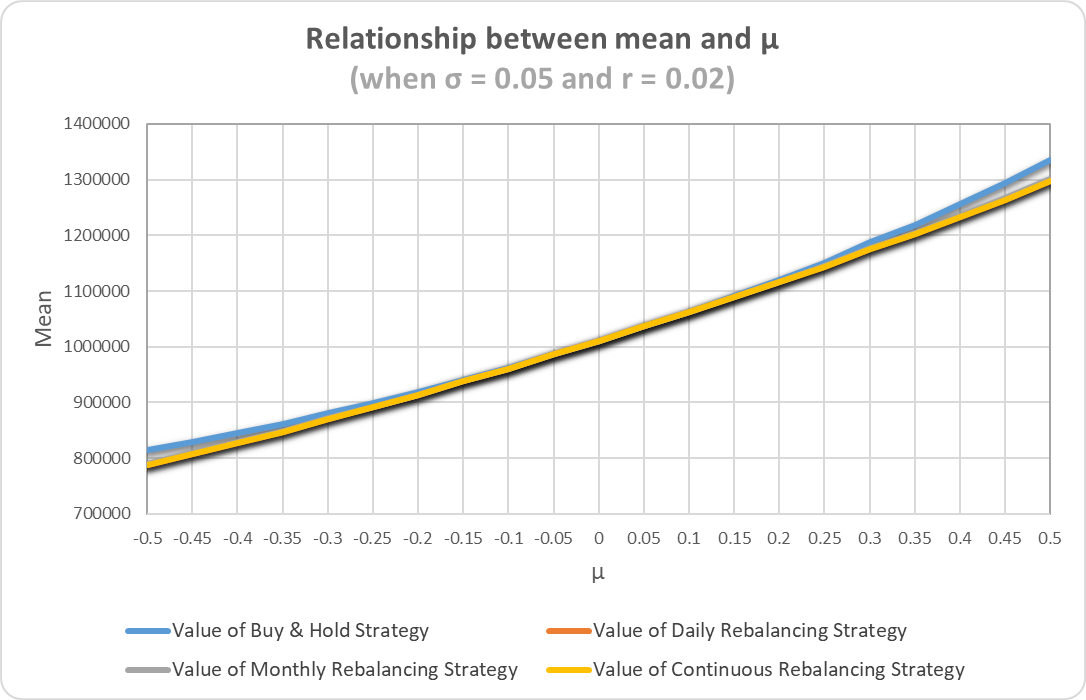
\includegraphics[width=0.7\linewidth]{mean_mu_005_002}
	\caption{}
	\label{fig:meanmu005002}
\end{figure}
As we can see from Figure 1, the Y-axis represents the mean of the portfolio value at time T, and the X-axis represents the parameter $\mu$ which is used in the simulation. We fixed $\sigma$ at 0.05 and $r$ at 0.02.\\

Overall, the buy-and-hold and rebalancing strategies have almost the same positive relationships between portfolio's mean value and $\mu$ . The subtle differences exist when the absolute values of $\mu$ are larger, and then buy-and-hold has the larger value of mean than rebalancing. When $\mu$ is close to 0, the advantage of buy-and-hold diminishes, and rebalancing performs slightly better.\\

The explanation for this phenomena is that when the $\mu$ of the risk asset is very high, the risk asset keeps creating value for the whole portfolio, and rebalance will decrease the weight of the profitable risk asset hence decreasing the value of the portfolio. When the $\mu$ is very low, however, the value and weight of the risk asset keep decreasing over the time. If the portfolio is rebalanced, the weight of risk asset is enlarged and higher loss for the portfolio is likely to occur.\\

We also find that the relative relationship between the mean of the portfolio and $\mu$ is not sensitive to the change of $\sigma$ and $r$. They all show the similar pattern as in Figure 1.\\

\begin{figure}[H]
	\centering
	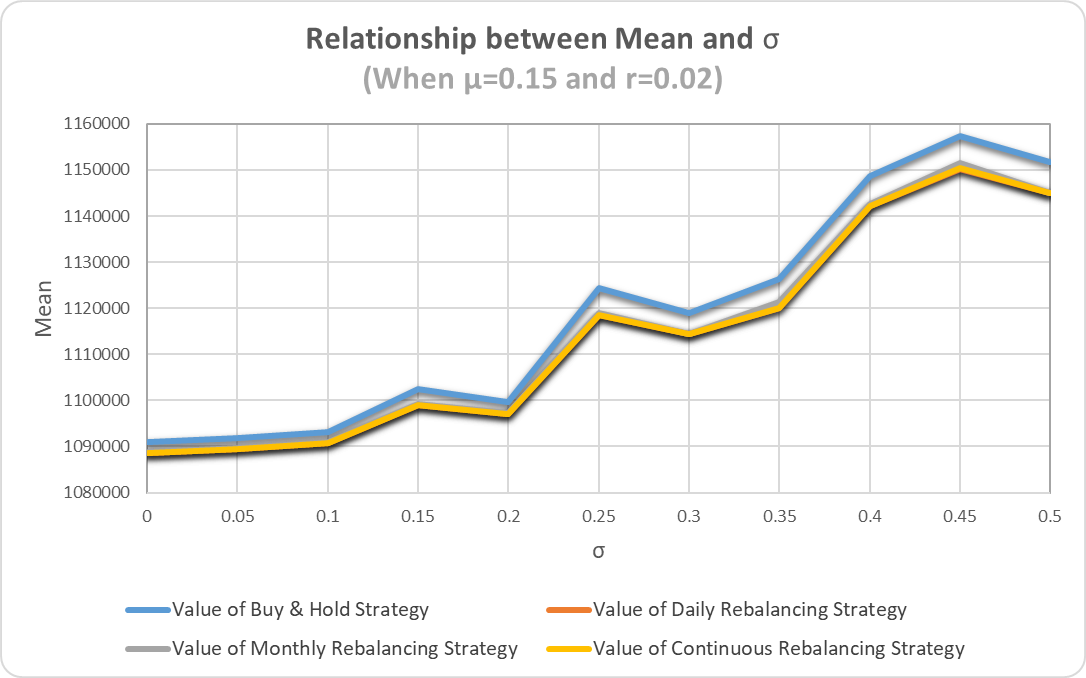
\includegraphics[width=0.7\linewidth]{mean_sigma_015_002}
	\caption{}
	\label{fig:meansigma015002}
\end{figure}
For Figure 2, the Y-axis represents the mean of the portfolio value at time T, and the X-axis represents the parameter $\sigma$ which is used in the simulation. We fixed $\mu$ at 0.15 and $r$ at 0.02.\\

The two different kinds of strategies have the same pattern of relationships between mean and $\sigma$. When $\sigma$ goes from 0 to 0.5, mean would follow an uptrend. The buy-and-hold strategy has bigger mean value than rebalancing strategies at every point of $\sigma$. \\

\begin{figure}[H]
	\centering
	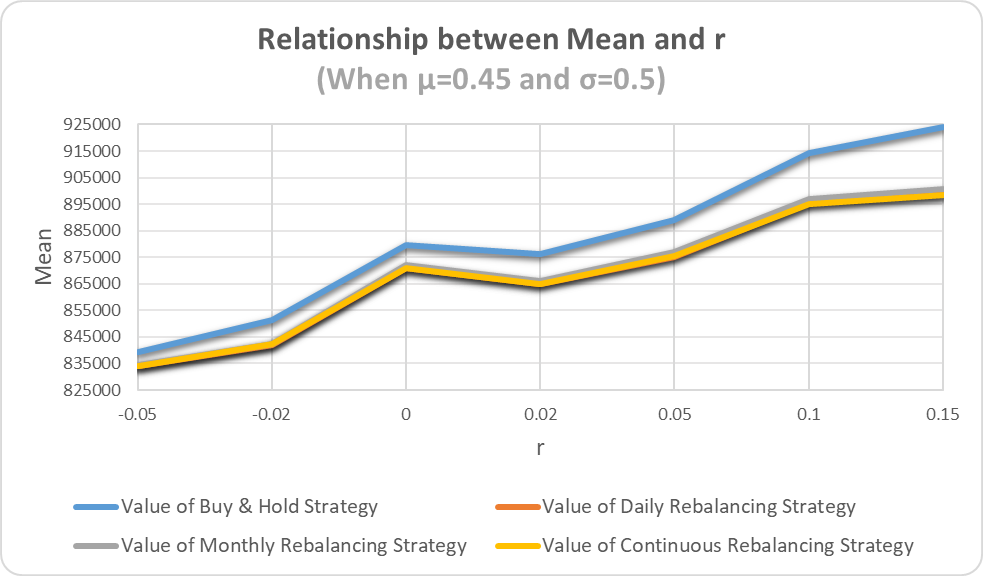
\includegraphics[width=0.7\linewidth]{mean_r_045_050}
	\caption{}
	\label{fig:meanr045050}
\end{figure}

For Figure 3, the Y-axis represents the mean of the portfolio value at time T, and the X-axis represents the parameter r which is used in the simulation. We fixed $\mu$ at 0.45 and $\sigma$ at 0.5.\\

The two different kinds of strategies have the same pattern of relationships between mean and $r$. However, the buy-and-hold strategy has bigger mean value than rebalancing strategies at every point of $r$. Under the circumstances of same $\sigma$, the overall difference between the two different kinds of strategies is bigger if the $r$ is bigger. \\



\begin{figure}[H]
	\centering
	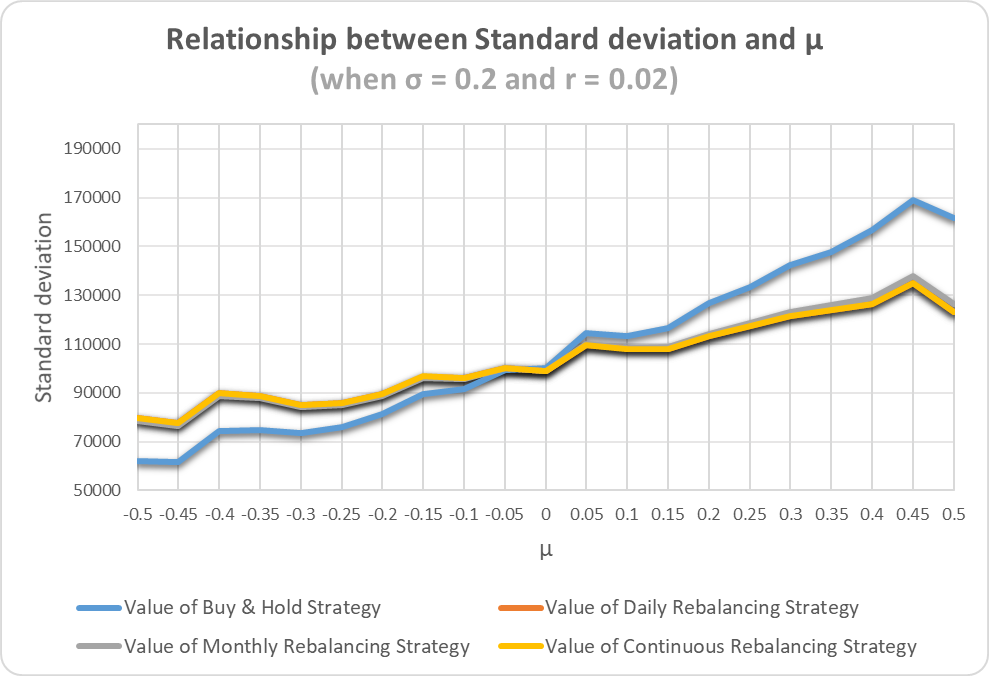
\includegraphics[width=0.7\linewidth]{std_mu_020_002}
	\caption{}
	\label{fig:stdmu020002}
\end{figure}
For Figure 4, the Y-axis represents the standard deviation of the portfolio value at time T, and the X-axis represents the parameter $\mu$ which is used in the simulation. We fixed $\sigma$ at 0.2 and $r$ at 0.02.\\

As $\mu$ goes up, the standard deviation will increase correspondingly which indicates that a bull market would lead to more deviation than a bear market.  Also, when $\mu$ is less than 0, the standard deviation of buy-and-hold strategy is less than rebalancing strategy. Whereas when $\mu$ is higher than 0, the standard deviation of buy-and-hold strategy is higher than rebalancing strategy.\\ 

This pattern shows that buy-and-hold has less risk when the market is sluggish yet has more risk when the market is thriving. \\

\begin{figure}[H]
	\centering
	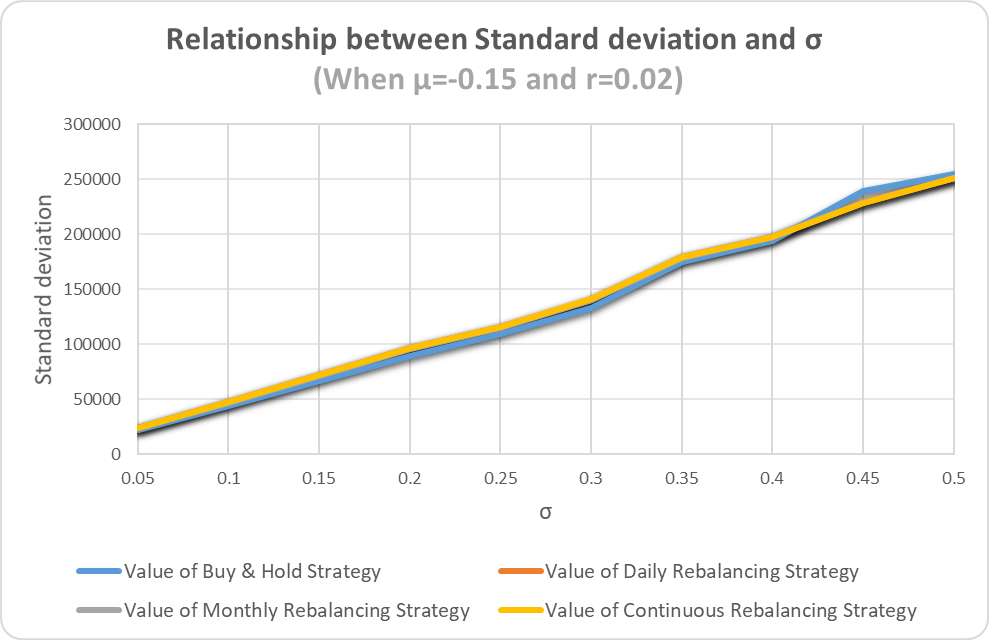
\includegraphics[width=0.7\linewidth]{std_sigma_-015_002}
	\caption{}
	\label{fig:stdsigma-015002}
\end{figure}

For Figure 5, the Y-axis represents the standard deviation of the portfolio value at time T, and the X-axis represents the parameter $\sigma$ which is used in the simulation. We fixed $\mu$ at -0.15 and $r$ at 0.02.\\

In this case, the standard deviation is highly positively correlated with $\sigma$ because the setting of $\sigma$ would have a big impact on the standard deviation of final results. Also, the difference between buy-and-hold strategy and rebalancing strategy is quite slim. \\


\begin{figure}[H]
	\centering
	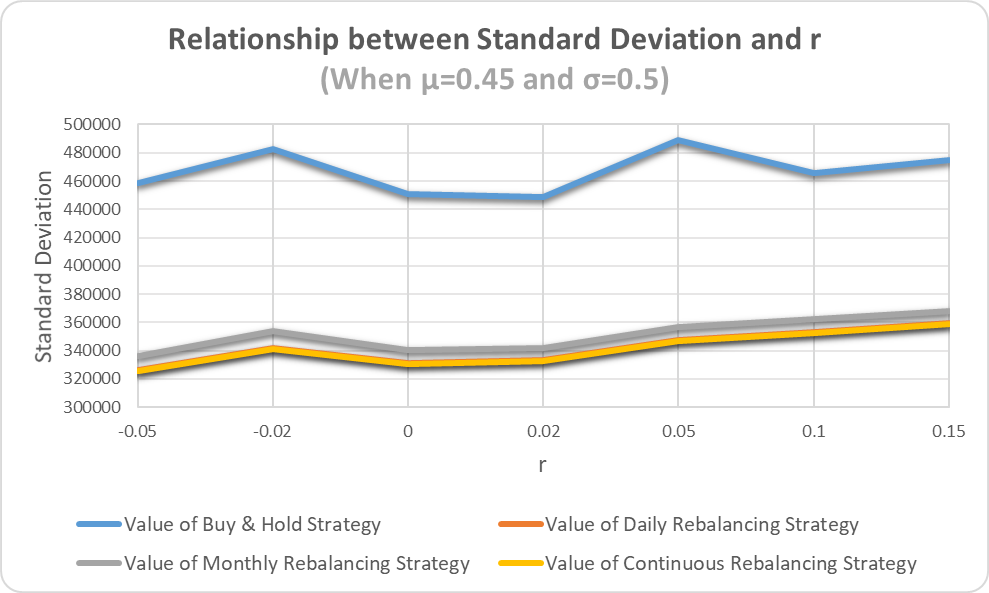
\includegraphics[width=0.7\linewidth]{std_r_045_050}
	\caption{}
	\label{fig:stdr045050}
\end{figure}

\begin{figure}[H]
	\centering
	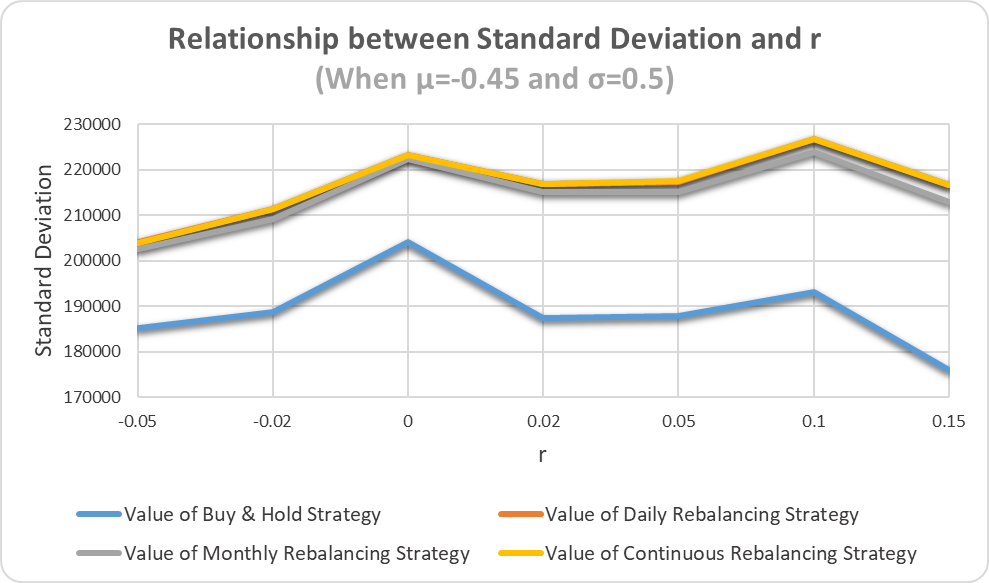
\includegraphics[width=0.7\linewidth]{std_r_-045_050}
	\caption{}
	\label{fig:stdr-045050}
\end{figure}
For Figure 6 and 7, the Y-axis represents the standard deviation of the portfolio value at time T, and the X-axis represents the parameter $r$ which is used in the simulation. We fixed $\mu$ at 0.45(figure 6), -0.45(figure 7) and $\sigma$ at 0.02(both).\\

Standard deviation doesn’t change a lot as the variation of interest rate which means $r$ doesn't have a certain impact on the standard deviation. Also, when $\mu$ is above 0, which refers to an uptrend, the standard deviation of buy-and-hold strategy is higher than rebalancing strategy while when $\mu$ is below 0, which refers to a downtrend, the standard deviation of rebalancing strategy is higher than the buy-and-hold strategy. Consequently, different strategies indicate the function of risk management in a bullish or bearish market. \\

\begin{figure}[H]
	\centering
	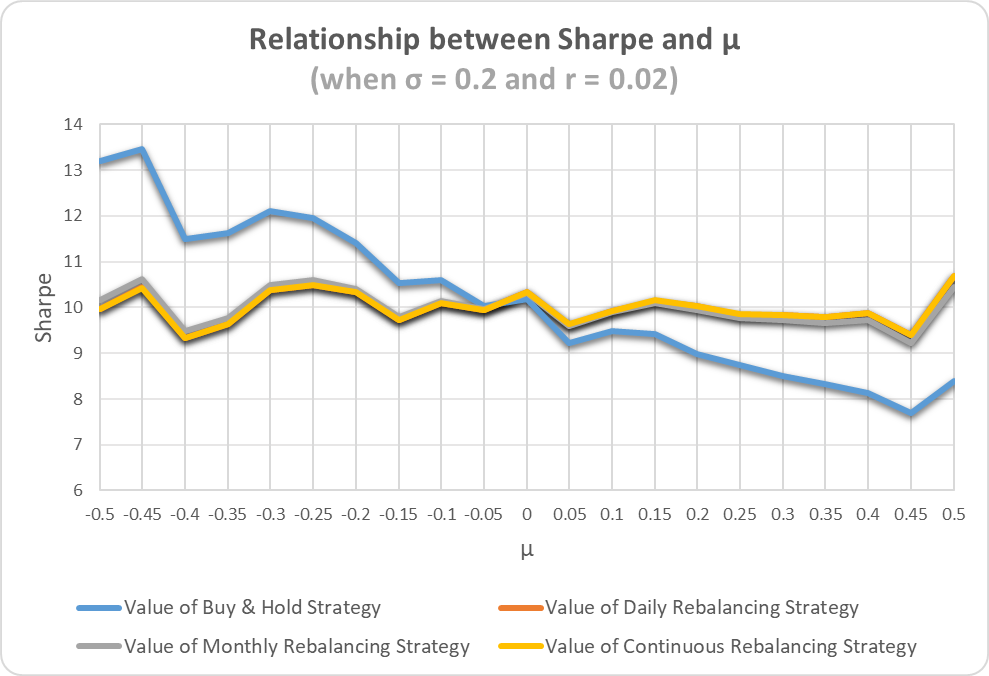
\includegraphics[width=0.7\linewidth]{sharpe_mu_020_002}
	\caption{}
	\label{fig:sharpemu020002}
\end{figure}
For Figure 8, the Y-axis represents the sharpe ratio of the portfolio value at time T, and the X-axis represents the parameter $\mu$ which is used in the simulation. We fixed $\sigma$ at 0.2 and $r$ at 0.02.\\

Sharpe ratio of buy and hold strategy decreases as $\mu$ increases while sharpe ratio of rebalancing strategy almost remains the same. Thus, when $\mu$ is less than 0, the buy-and-hold strategy has bigger sharpe value than rebalancing strategies. When $\mu$ is more than 0, the buy-and-hold strategy has smaller sharpe value than rebalancing strategies. \\

Sharpe ratio measures risk-adjusted return. When comparing figure 9 with figure 1, we notice that the buy-and-hold strategy has higher risk-adjusted return when $\mu$ goes to -0.5 and rebalancing strategy outperforms buy and hold strategy in terms of risk-adjusted return when $\mu$ goes to 0.5.


\begin{figure}[H]
	\centering
	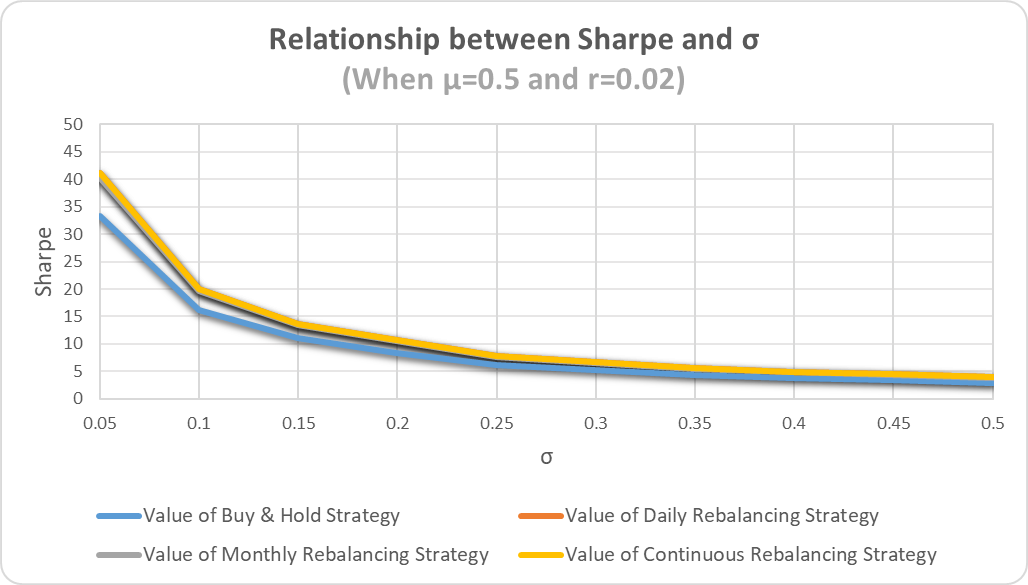
\includegraphics[width=0.7\linewidth]{sharpe_sigma_050_002}
	\caption{}
	\label{fig:sharpesigma050002}
\end{figure}

\begin{figure}[H]
	\centering
	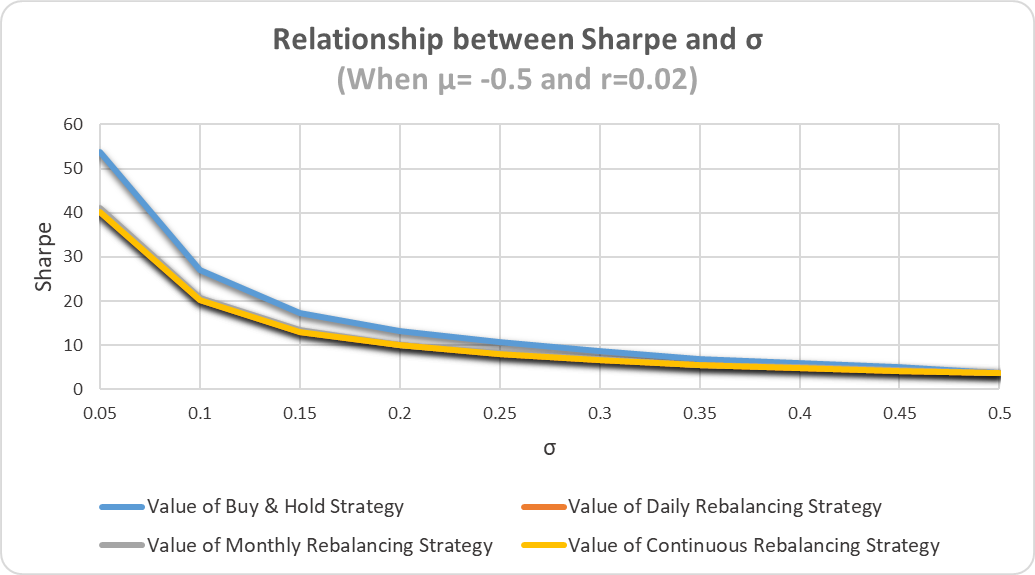
\includegraphics[width=0.7\linewidth]{sharpe_sigma_-050_002}
	\caption{}
	\label{fig:sharpesigma-050002}
\end{figure}
For Figure 9 and 10, the Y-axis represents the sharpe ratio of the portfolio value at time T, and the X-axis represents the parameter $\sigma$ which is used in the simulation. We fixed $\mu$ at 0.5(figure 9), -0.5(figure 10) and $r$ at 0.02(both).\\

As $\sigma$ goes up, sharpe ratio goes down and it resembles an exponential function. When $\sigma$ is close to 0.05, sharpe ratio is quite large yet when $\sigma$ goes to 0.5, sharpe ratio approaches 0. Similarly, the difference between buy-and-hold strategy and rebalancing strategy is big when $\sigma$ is small and vice versa.\\

This pattern indicates that when $\sigma$ increases even slightly sharpe ratio would decrease dramatically because of the standard deviation of the portfolio.\\

\begin{figure}[H]
	\centering
	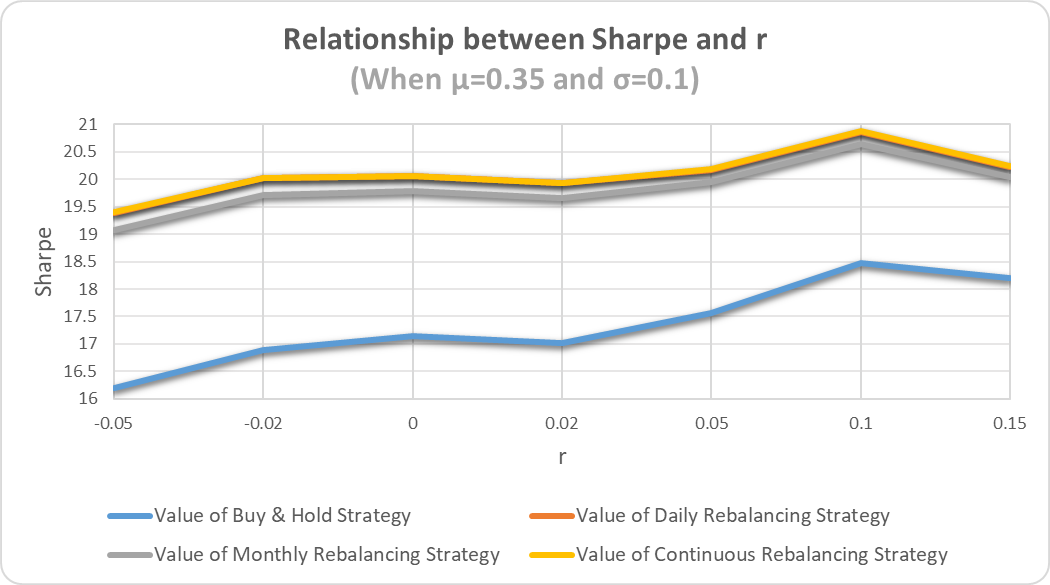
\includegraphics[width=0.7\linewidth]{sharpe_r_035_010}
	\caption{}
	\label{fig:sharper035010}
\end{figure}

\begin{figure}[H]
	\centering
	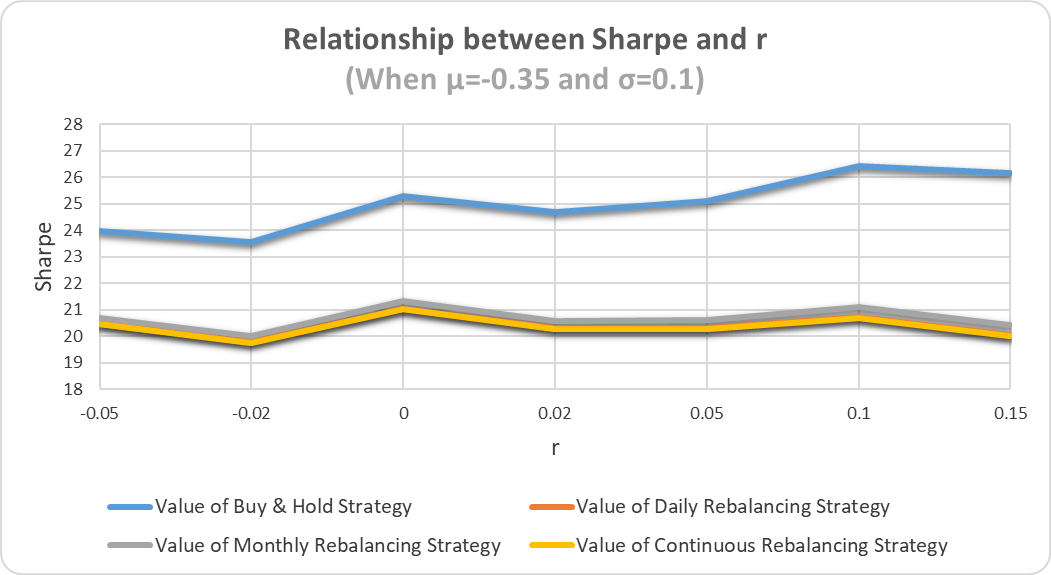
\includegraphics[width=0.7\linewidth]{sharpe_r_-035_010}
	\caption{}
	\label{fig:sharper-035010}
\end{figure}
For Figure 11 and 12, the Y-axis represents the sharpe ratio of the portfolio value at time T, and the X-axis represents the parameter $r$ which is used in the simulation. We fixed $\mu$ at 0.35(figure 11), -0.35(figure 12) and $\sigma$ at 0.1(both).\\

{\tiny When interest rate increases, sharpe ratio doesn’t increase a lot and the plot is quite flat. However,  when $\mu$ is higher than 0, sharpe ratio of rebalancing strategy is higher than that of buy-and-hold strategy. When $\mu$ is less than 0, sharpe ratio of rebalancing strategy is less than that of buy-and-hold strategy. It implies that risk-adjusted return is higher for rebalancing strategy in a bullish market. }\\

\begin{figure}[H]
	\centering
	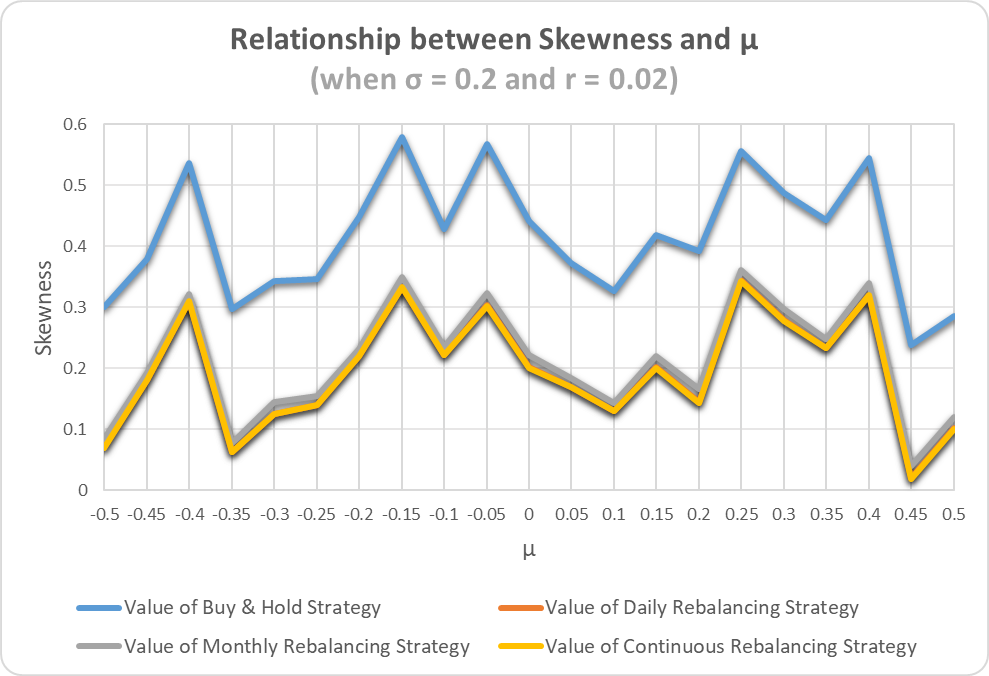
\includegraphics[width=0.7\linewidth]{skew_mu_020_002}
	\caption{}
	\label{fig:skewmu020002}
\end{figure}
For Figure 13, the Y-axis represents the skewness of the portfolio value at time T, and the X-axis represents the parameter $\mu$ which is used in the simulation. We fixed $\sigma$ at 0.2 and $r$ at 0.02.\\

There is no trend between skewness and $\mu$ and skewness of buy-and-hold strategy is higher than that of rebalancing strategy. Since skewness is a measure of symmetry and positive skew means the long tail is on the positive side of the peak, all strategies show the pattern of right skewness and buy-and-hold strategy is more obvious than rebalancing strategy.\\

\begin{figure}[H]
	\centering
	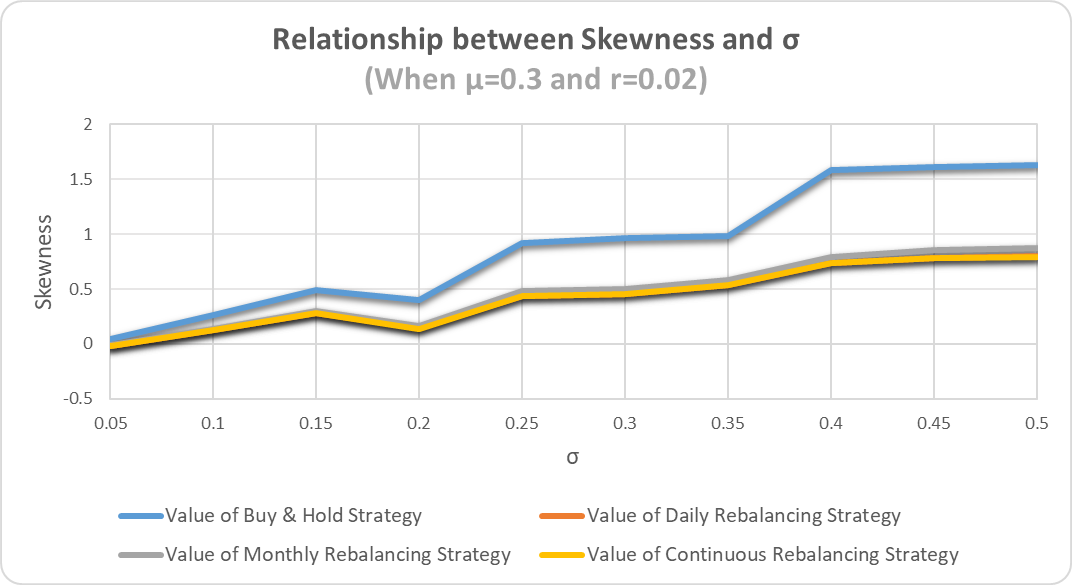
\includegraphics[width=0.7\linewidth]{skew_sigma_030_002}
	\caption{}
	\label{fig:skewsigma030002}
\end{figure}
For Figure 14, the Y-axis represents the skewness of the portfolio value at time T, and the X-axis represents the parameter $\sigma$ which is used in the simulation. We fixed $\mu$ at 0.3 and $r$ at 0.02.\\

Skewness will increase slightly as $\sigma$ increases and skewness is above 0. Skewness of buy-and-hold strategy is a little higher than that of rebalancing strategy and as discussed before, they are all right-skewed.\\

\begin{figure}[H]
	\centering
	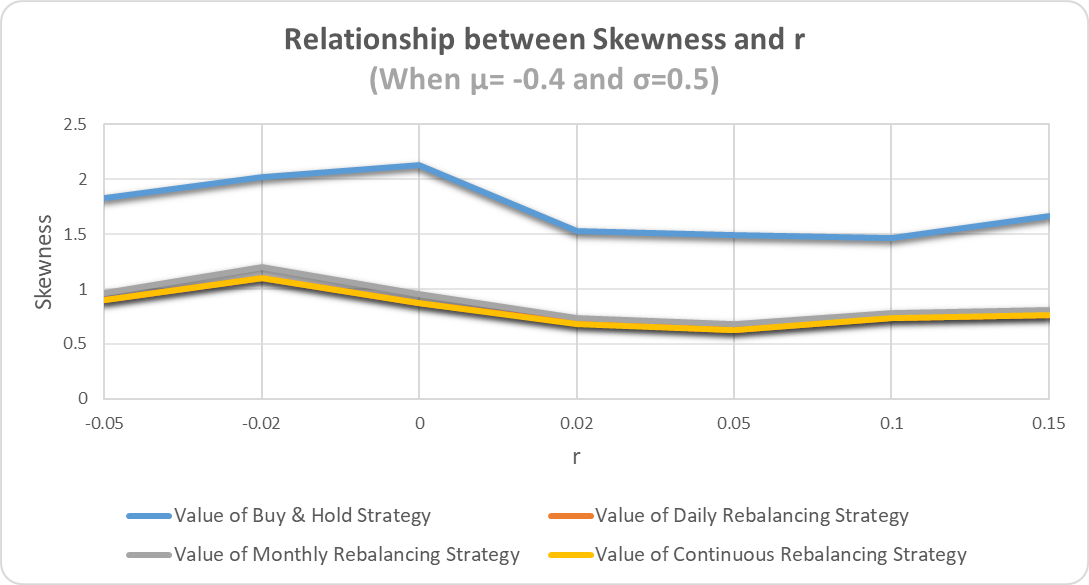
\includegraphics[width=0.7\linewidth]{skew_r_-040_050}
	\caption{}
	\label{fig:skewr-040050}
\end{figure}
For Figure 15, the Y-axis represents the skewness of the portfolio value at time T, and the X-axis represents the parameter $r$ which is used in the simulation. We fixed $\mu$ at -0.4 and $\sigma$ at 0.5.\\

The chart shows that skewness doesn’t change a lot with the change of interest rate. And skewness of buy-and-hold strategy is higher than that of rebalancing strategy which means the buy-and-hold strategy is more positive skew. \\

\begin{figure}[H]
	\centering
	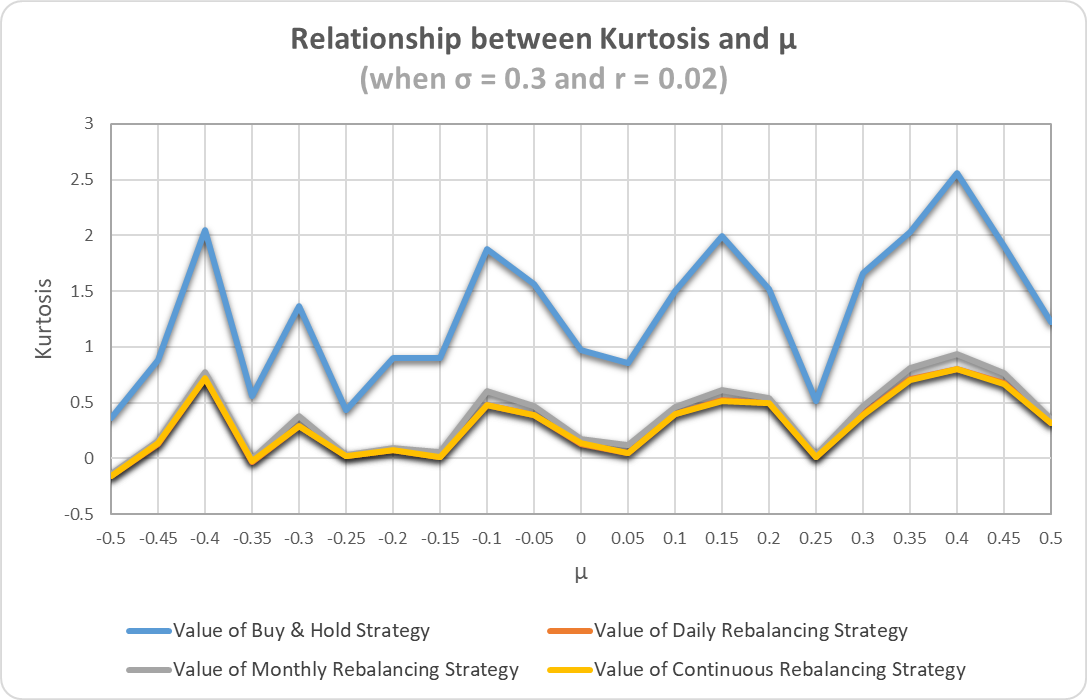
\includegraphics[width=0.7\linewidth]{Kurto_mu_030_002}
	\caption{}
	\label{fig:kurtomu030002}
\end{figure}
For Figure 16, the Y-axis represents the kurtosis of the portfolio value at time T, and the X-axis represents the parameter $\mu$ which is used in the simulation. We fixed $\sigma$ at 0.3 and $r$ at 0.02.\\

All the plots under different $\sigma$’s and r’s show that the Kurtosis value for buy-and-hold strategy is higher than the rebalancing strategies. And there is no clear pattern between $\mu$ and kurtosis, the relationship is quite random. All the strategies have the kurtosis less than 3, which means that they are Platykurtic. The frequency of rebalancing strategies doesn’t have too much impact on the Kurtosis. \\



\begin{figure}[H]
	\centering
	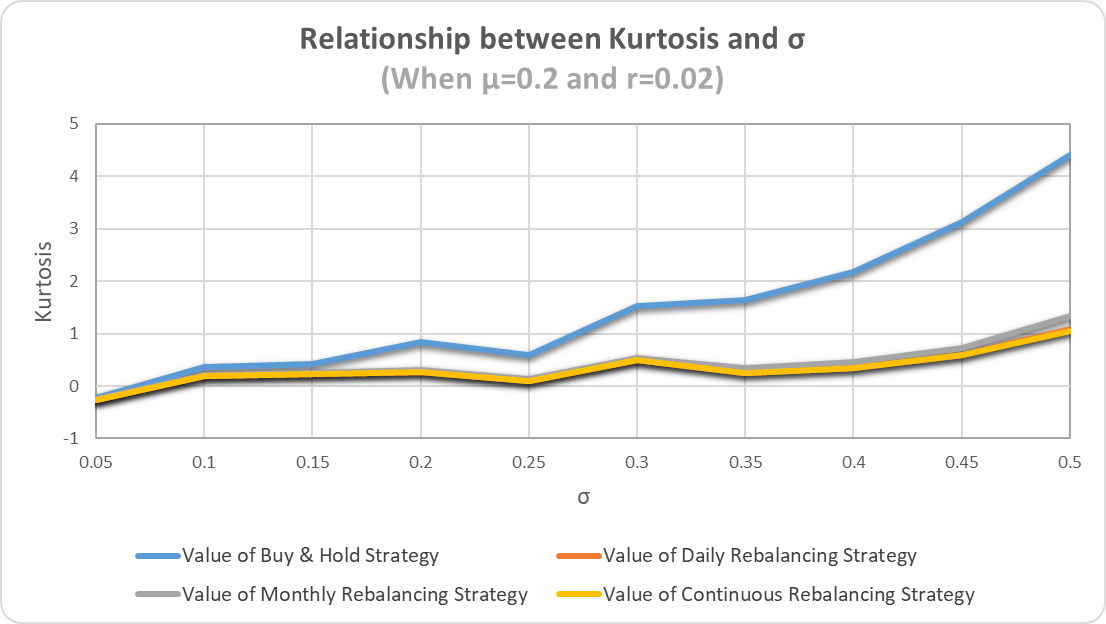
\includegraphics[width=0.7\linewidth]{Kurto_sigma_020_002}
	\caption{}
	\label{fig:kurtosigma020002}
\end{figure}
For Figure 17, the Y-axis represents the kurtosis of the portfolio value at time T, and the X-axis represents the parameter $\sigma$ which is used in the simulation. We fixed $\mu$ at 0.2 and $r$ at 0.02.\\

From this plot, we could see that when $\mu$ and r are fixed, as $\sigma$ becomes bigger, all the strategies' kurtosis becomes bigger also. Overall, the rebalancing strategies’ Kurtosis is bigger than buy-and-hold strategies and the difference between buy-and-hold and rebalancing increases as $\sigma$ grows.\\
\begin{figure}[H]
	\centering
	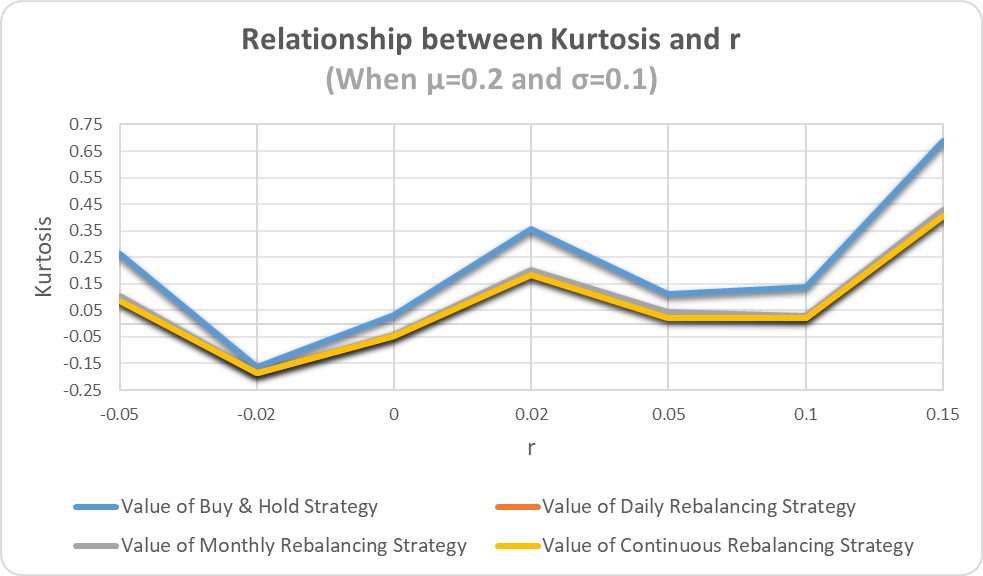
\includegraphics[width=0.7\linewidth]{Kurto_r_020_010}
	\caption{}
	\label{fig:kurtor020010}
\end{figure}


\begin{figure}[H]
	\centering
	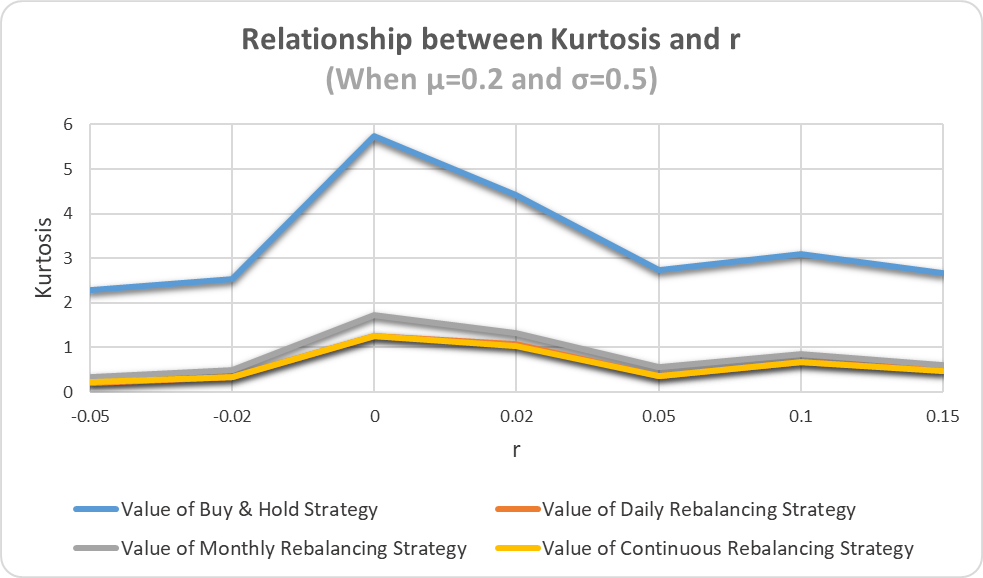
\includegraphics[width=0.7\linewidth]{Kurto_r_020_050}
	\caption{}
	\label{fig:kurtor020050}
\end{figure}
For Figure 18 and 19, the Y-axis represents the kurtosis of the portfolio value at time T, and the X-axis represents the parameter $r$ which is used in the simulation. We fixed $\mu$ at 0.2(both) and $\sigma$ at 0.1(figure 19), 0.5(figure 20).\\

All the plots under different $\sigma$’s and $\mu$’s show that the Kurtosis value for buy-and-hold strategy is higher than the rebalancing strategies. And there is also no clear pattern between r and kurtosis, the relationship is quite random. Comparing the plot with same $\mu$ and different $\sigma$, we can find that the difference between buy-and-hold strategy and rebalancing strategies are bigger if $\sigma$ is bigger. The frequency of rebalancing strategies doesn’t have too much impact on the Kurtosis. \\


\subsection{Historical Analysis}
We then use historical data to validate our findings from simulation.
\begin{figure}[H]
	\centering
	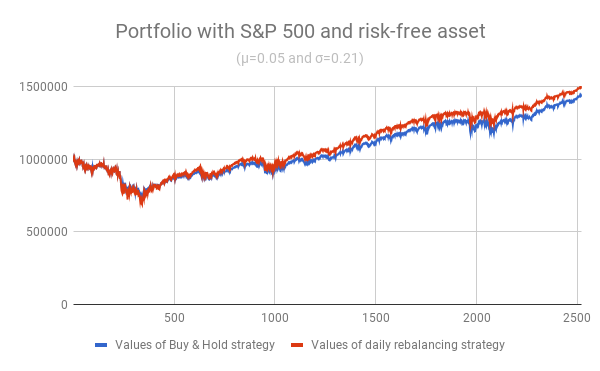
\includegraphics[width=0.7\linewidth]{sp500}
	\caption{}
	\label{fig:sp500}
\end{figure}
As we can see from Figure 20, the X-axis represents time and Y-axis represents the value of the portfolio at each point of the time. During the backtest period, the estimated $\mu$ of SP500 is 0.05, and its estimated $\sigma$ is 0.21. \\

We can see from this graph that the rebalance strategy beats buy-and-hold strategy at time T. But the spread between these two is relatively low. This is in accordance with the pattern shown in Figure 1 which is drawn under $\sigma = 0.05$ and $r = 0.02$. (We have mentioned earlier that the pattern is not sensitive to $\sigma$ and $r$). When the $\mu$ in Figure 1 is close to 0.05, rebalancing performs better than buy-and-hold. This is in harmony with the results in Figure 20.\\

\begin{figure}[H]
	\centering
	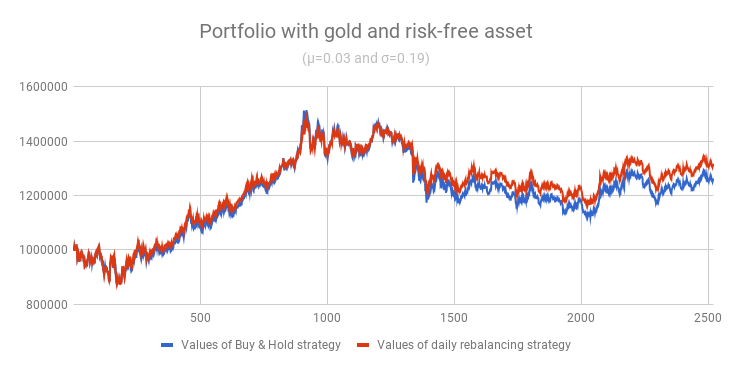
\includegraphics[width=0.7\linewidth]{gold}
	\caption{}
	\label{fig:gold}
\end{figure}

The same is true with gold, as shown in Figure 21. When the $\mu$ is close to 0, rebalancing usually performs slightly better than buy-and-hold at time T.\\

\begin{figure}[H]
	\centering
	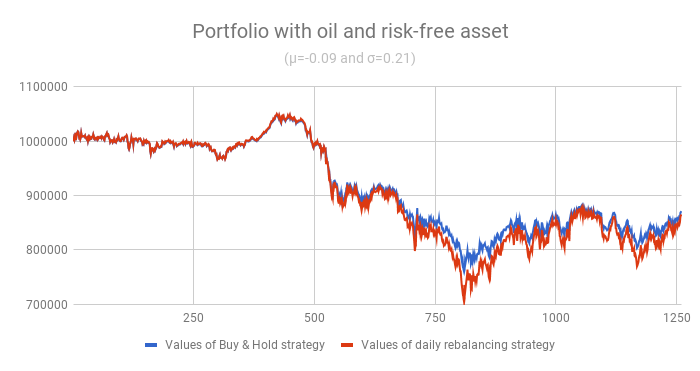
\includegraphics[width=0.7\linewidth]{oil}
	\caption{}
	\label{fig:oil}
\end{figure}

For oil market, however, the situation is different. As we can see from Figure 22, its $\mu$ is -0.09 which is farther from 0 than SP500 and gold. And it is shown that the buy-and-hold slightly beat rebalancing in the end, which also validates our conclusion from the simulation.

\subsection{New Approach Analysis}
As we can see from the simulation analysis and the historical analysis, both buy-and-hold and rebalancing strategies have advantages over one another under some certain market scenarios. Here, based on our previous analysis, we are going to propose another new approach for rebalancing which also shows its superior features under some specific situations.\\

This new approach uses some predetermined criteria to trigger rebalancing signals. For example, when the wight of risk asset is higher than 60\%, we rebalance its weight back to its original 50\%. We could make the criteria even more complex, based on how we interpret the market.\\

To better understand the feature of this strategy, we select a special scenario where $\mu = 0$ and $\sigma = 0.50$. This is typically a mean-reversion market with high volatility. Intuitively, it seems wise to increase the weight of the risk asset when its price falls under some level in case it goes up in the short future, and decrease the weight when some gains have already been made. \\

\begin{figure}[H]
	\centering
	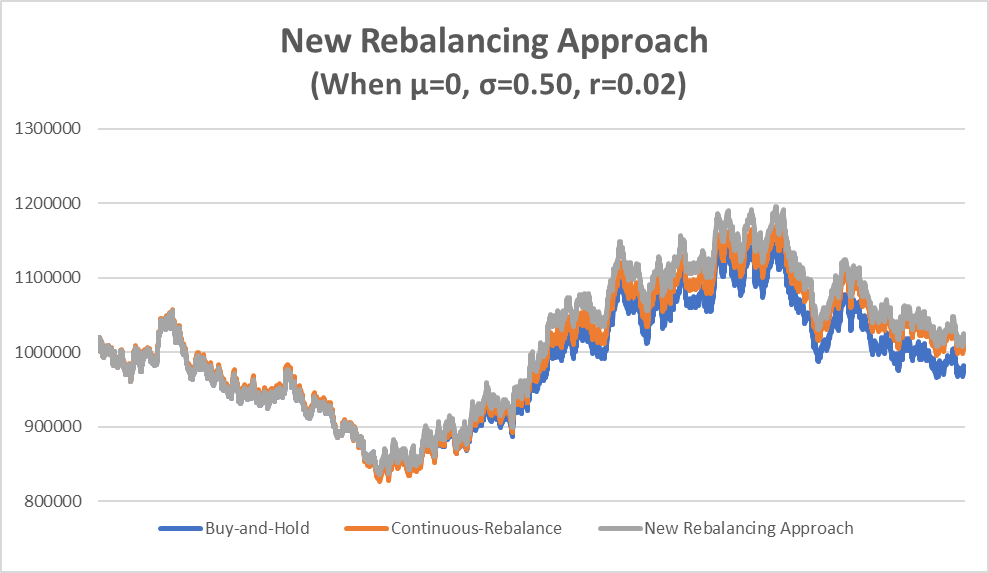
\includegraphics[width=0.7\linewidth]{newApproach}
	\caption{}
	\label{fig:newapproach}
\end{figure}

Figure 23 shows that under this scenario, our new rebalancing approach performs better than other two strategies. This is also in accordance with our previous findings: when $\mu$ is close to 0, rebalancing performs better than buy-and-hold.\\

\begin{figure}[H]
	\centering
	\large
	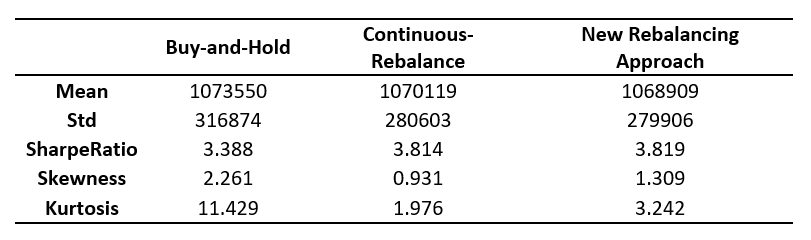
\includegraphics[width=1.0\linewidth]{newApproachTable}
	\caption{}
	\label{fig:newapproachtable}
\end{figure}

Figure 24 shows some statistics of the distribution under each strategy. The skewness and kurtosis of our new rebalancing approach are among those of the other two strategies. However, its Sharpe Ratio is the highest among all of them.\\

It is worth mentioning that our new rebalancing approach only rebalances a few times during the whole simulation period, which dramatically reduces transaction costs compared to continuous rebalancing.\\

\subsection{Summary}

To sum up, both buy-and-hold strategy and rebalancing strategy have its advantages under specific market scenarios. As for portfolio returns, buy-and-hold usually beats rebalancing when the risk asset return $\mu$ is too high and too low; while rebalancing shows its advantage when $\mu$ is close to 0 (See Figure 1). As for the risk-adjusted return, however, (as we can see from Figure 8), the Sharpe ratio of rebalancing is stable no matter what the $\mu$ is, while the Sharpe ratio of buy-and-hold decreases with the increase of $\mu$. We also find that the frequency of rebalancing does not matter too much.\\

We use historical data to further support our findings in the simulation. We find that in either stock market, gold market or oil market, over the past 20 years, our simulation results are applicable. This indicates the correctness of our simulation model as well as the results we find in the simulation.\\

At last, based on our observation of the simulation results and intuition about the market, we propose another new rebalancing approach which use some predetermined criteria to trigger rebalance signals. It shows its superior advantage under some extreme situations. Generally, it has performance between the other two strategies. However, we have yet to take into consideration the transaction costs which may dramatically decrease the performance of high-frequent rebalancing. As a result, our new rebalancing approach may be a better choice than traditional rebalancing. 






%----------------------------------------------------------------------------------------
%	BIBLIOGRAPHY
%----------------------------------------------------------------------------------------

\renewcommand{\refname}{\spacedlowsmallcaps{References}} % For modifying the bibliography heading

\bibliographystyle{apalike}

\bibliography{references} % The file containing the bibliography



%----------------------------------------------------------------------------------------

\end{document}